\documentclass[11pt]{beamer}
\usetheme{Rochester}
\usepackage{amsmath} %основной пакет для формул
\usepackage[utf8]{inputenc}
\usepackage[english,russian]{babel}
\usepackage[OT1]{fontenc}
\usepackage{amsfonts}
\usepackage{amssymb}
\usepackage{here}
\usepackage{hyperref}
\beamertemplatenavigationsymbolsempty
\author{Дьячков Вадим Вадимович\\
Жуйков Артём Александрович\\
Ламтев Антон Юрьевич\\
Леженин Юрий Игоревич\\}
\title[Методы сжатия изображений]{Методы сжатия изображений}
\setbeamercovered{transparent} 
%\setbeamertemplate{navigation symbols}{} 
%\logo{} 
\institute{Санкт-Петербургский политехнический университет Петра Великого\\
Институт компьютерных наук и технологий\\
Кафедра компьютерных систем и программных технологий\\
Группа 13501/4} 
\date{\the\year}
\begin{document}


\begin{frame}
\titlepage
\end{frame}


%\begin{frame}{Актуальность темы}
%\begin{itemize}
%	\item повседневное использование людьми сжатых изображений
%	\item 
%\end{itemize}
%\end{frame}


\begin{frame}{Методы сжатия}
\begin{itemize}
	\item С потерями
	\begin{itemize}
		\item Квантование и дискретизация
		\item Цветовое пространство $YC_bC_r$ и цветовая субдискретизация
		\item Вейвлет сжатие
		\item Дискретное косинусное преобразование
	\end{itemize}
	\item Без потерь
	\begin{itemize}
		\item Алгоритм Хаффмана
		\item Алгоритм LZW
		\item Алгоритм RLE
	\end{itemize}
\end{itemize}
\end{frame}



\begin{frame}{Дискретизация}
\begin{block}{Уменьшение точности дискретизации}
\begin{figure}[H]
	\begin{center}
		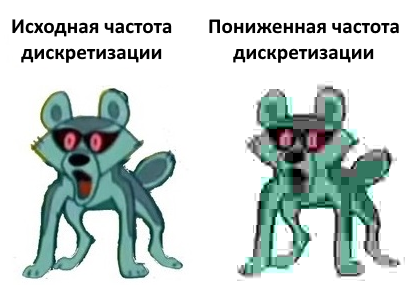
\includegraphics[scale=0.73]{../pics/quantization/shakal.png}
		%\caption{Уменьшение точности дискретизации} 
	\end{center}
\end{figure}	
\end{block}				
\end{frame}



\begin{frame}{Квантование}
\begin{block}{Уменьшение точности квантования}
\begin{figure}[H]
	\begin{center}
		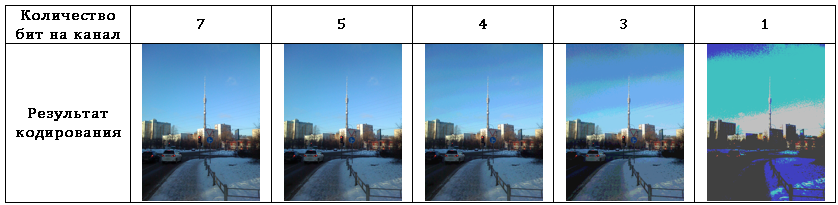
\includegraphics[scale=0.48]{../pics/quantization/quantization.png}
		%\caption{Уменьшение точности квантования} 
	\end{center}
\end{figure}	
\end{block}				
\end{frame}



\begin{frame}{Цветовое пространство $YC_bC_r$ и цветовая субдискретизация}
	\begin{displaymath}
		Y = k_rR + k_gG + k_bB
	\end{displaymath}

	\begin{center}
		$C_b = B - Y$

		$C_r = C - Y$

		$C_g = G - Y$
	\end{center}
\end{frame}



\begin{frame}{Цветовое пространство $YC_bC_r$ и цветовая субдискретизация}
\begin{block}{Плоскость $YC_bC_r$ при постоянной яркости Y = 0.5}
\begin{figure}[H]
	\begin{center}
		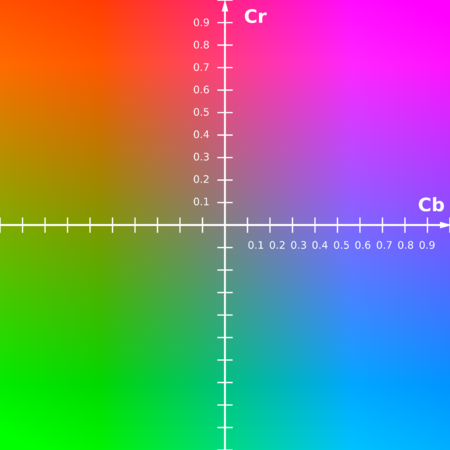
\includegraphics[scale=0.5]{../pics/YCbCr/YCbCr.png}
	\end{center}
	%\center{Плоскость $YC_bC_r$ при постоянной яркости Y = 0.5}
\end{figure}	
\end{block}			
\end{frame}



\begin{frame}{Цветовое пространство $YC_bC_r$ и цветовая субдискретизация}
\begin{block}{Цветное изображение и его компоненты Y, $C_B$ и $C_R$}
\begin{figure}[H]
	\begin{center}
		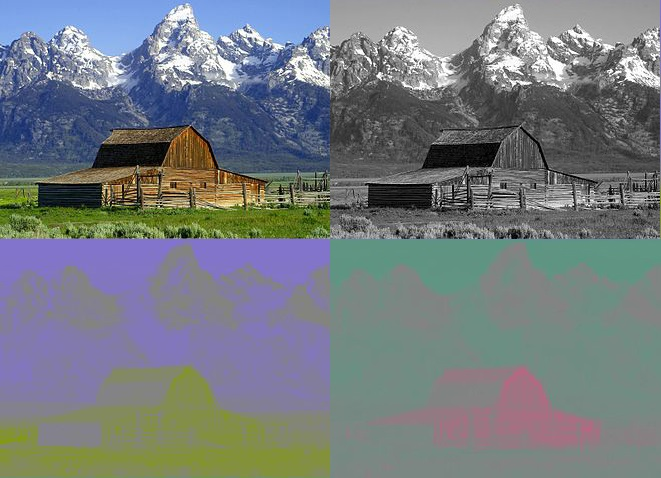
\includegraphics[scale=0.77]{../pics/YCbCr/YCbCr_separation_vert.jpg}
	\end{center}
	%\center{Цветное изображение и его компоненты Y, $C_B$ и $C_R$}
\end{figure}
\end{block}
\end{frame}



\begin{frame}{Цветовое пространство $YC_bC_r$ и цветовая субдискретизация}
\begin{block}{Форматы субдискретизации}
\begin{figure}[H]
	\begin{center}
		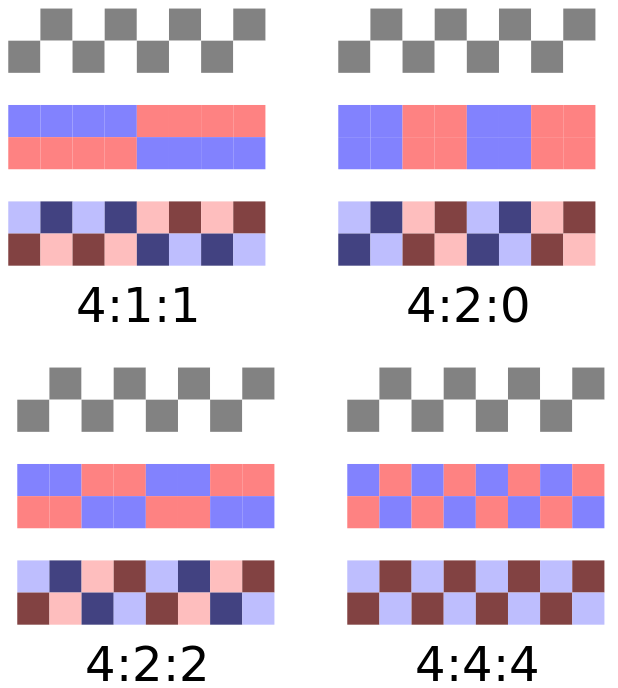
\includegraphics[scale=0.38]{../pics/chroma_subsampling/chroma_subsampling_ratios_pr.png}
		%\center{Форматы субдискретизации}
	\end{center}
\end{figure}	
\end{block}				
\end{frame}



\begin{frame}{Вейвлет сжатие}
\begin{block}{Одномерное преобразование Хаара}
\begin{figure}[H]
	\begin{center}
		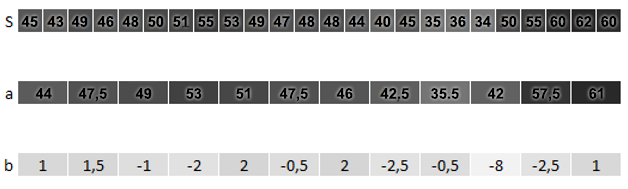
\includegraphics[scale=0.65]{../pics/wavelet/example.png}
		%\caption{Пример для одномерного пространства} 
	\end{center}
\end{figure}	
\end{block}				
\end{frame}



\begin{frame}{Вейвлет сжатие}
\begin{block}{Двумерное преобразование Хаара. Сжатие}
\begin{figure}[H]
	\begin{center}
		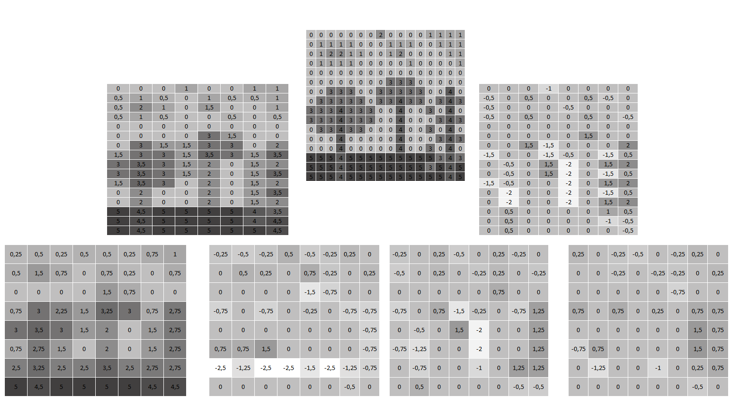
\includegraphics[scale=0.53]{../pics/wavelet/compression_pr.png}
		%\caption{Процесс сжатия} 
	\end{center}
\end{figure}	
\end{block}				
\end{frame}



\begin{frame}{Вейвлет сжатие}
\begin{block}{Двумерное преобразование Хаара. Восстановление}
\begin{figure}[H]
	\begin{center}
		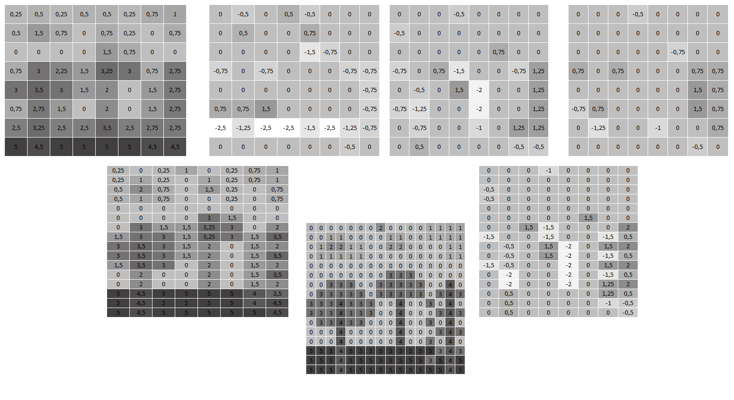
\includegraphics[scale=0.53]{../pics/wavelet/uncompression_pr.png}
		%\caption{Процесс восстановления} 
	\end{center}
\end{figure}	
\end{block}				
\end{frame}



\begin{frame}{Дискретное косинусное преобразование}
\begin{block}{Комбинация горизонтальных и вертикальных частот}
\begin{figure}[H]
	\begin{center}
		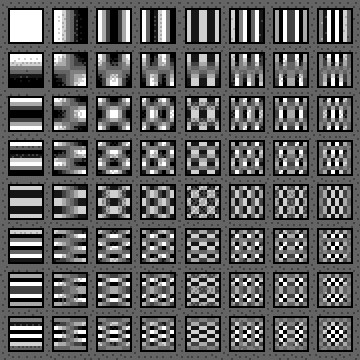
\includegraphics[scale=0.35]{../pics/cosine_transform/matrix.png}
		%\caption{Процесс и результат кодирования}
	\end{center}
\end{figure}	
\end{block}				
\end{frame} 



\begin{frame}{Алгоритм Хаффмана}
\begin{block}{Бинарное дерево Хаффмана для слова "КУКУШКА"}
\begin{figure}[H]
	\begin{center}
		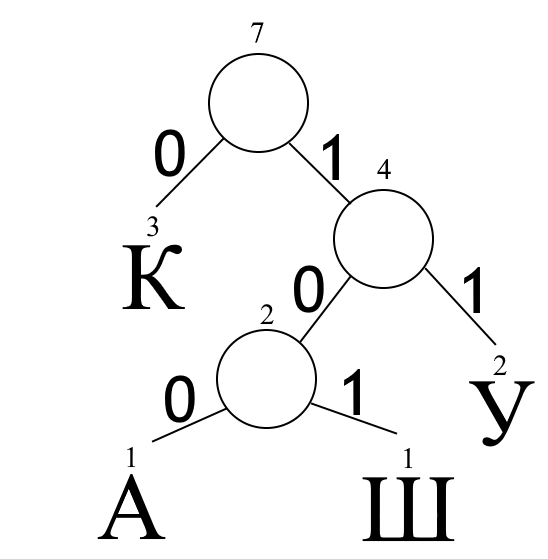
\includegraphics[scale=0.42]{../pics/Huffman/huffman.png}
		%\caption{Бинарное дерево Хаффмана}
	\end{center}
\end{figure}	
\end{block}				
\end{frame}



\begin{frame}{Алгоритм LZW}
\begin{block}{Начальный словарь}
%\begin{figure}[H]
%	\begin{center}
%		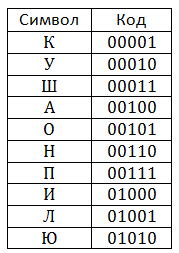
\includegraphics[scale=0.8]{../pics/LZW/dictionary.png}
%		%\caption{Начальный словарь}
%	\end{center}
%\end{figure}
\renewcommand{\arraystretch}{1.5}
\begin{table}[H]
\begin{center}
	\begin{tabular}{|c|c|}
		\hline	
		Символ & Код \\
		\hline
		  К    & 0001 \\
		\hline
		  У	   & 0010 \\
		\hline  
	  	  Ш	   & 0011 \\
		\hline  	
		  А    & 0100 \\
		\hline
	\end{tabular}
	%\caption{Начальный словарь}
\end{center}
\end{table}
\end{block}				
\end{frame}


 
\begin{frame}{Алгоритм LZW}
\begin{block}{Процесс и результат кодирования}
%\begin{figure}[H]
%	\begin{center}
%		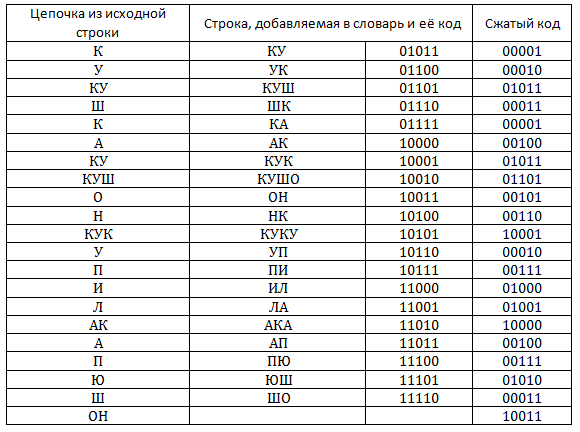
\includegraphics[scale=0.55]{../pics/LZW/result.png}
%		%\caption{Процесс и результат кодирования}
%	\end{center}
%\end{figure}
\begin{table}[H]
\begin{center}
	\begin{tabular}{|c|c|c|c|}
		\hline	
		  Цепочка из & \multicolumn{2}{|c|}{Строка, добавляемая в} & Сжатый \\
		  %подхачил малясь
		  исходной строки & \multicolumn{2}{|c|}{словарь и ее код} & код \\
		\hline
	  	  К    & КУ & 0101 & 0001 \\
		\hline
		  У	   & УК & 0110 & 0010 \\
		\hline  
		  КУ   & КУШ & 0111 & 0101 \\
		\hline  	
		  Ш    & ШК & 1000 & 0011 \\
		\hline
		  К    & КА & 1001 & 0001 \\
		\hline
		  А    &    &      & 0100 \\
		\hline
	\end{tabular}
	%\caption{Процесс и результат кодирования}
\end{center}
\end{table}
\end{block}				
\end{frame} 


\begin{frame}{Алгоритм RLE}
\begin{block}{Процесс и результат кодирования}
\begin{figure}[H]
	\begin{center}
		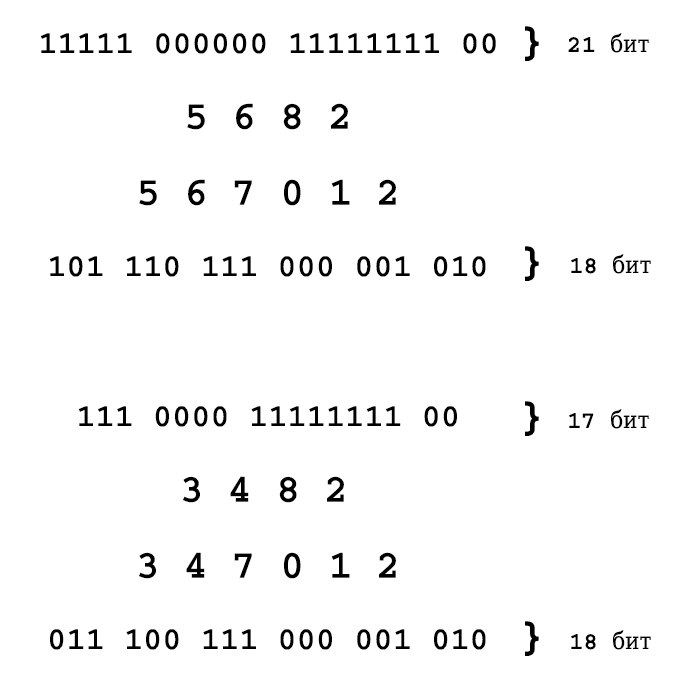
\includegraphics[scale=0.25]{../pics/RLE/example.jpg}
		%\caption{Процесс и результат кодирования}
	\end{center}
\end{figure}	
\end{block}				
\end{frame} 



\begin{frame}{Сжимаем аудиторию}
\begin{figure}[H]
	\begin{center}
		\huge\href{http://octo.ejiek.com/job/image_compression_algorithms/}{СЖАТЬ}
	\end{center}
\end{figure}					
\end{frame} 



\begin{frame}{}
\begin{center}
	\huge Спасибо за внимание!!!\\
	%
\includegraphics[scale=0.5]{../pics/smile.jpg}
\end{center}				
\end{frame}

\end{document}
